%% fig_annihilator.tex   (generated by make_core.py; do not edit by hand)
%% H^{0,2} in three blocks at n = 3: the outer two are carried injectively, the middle one of dimension n^2 goes to zero.
\documentclass[tikz,border=8pt]{standalone}
\usepackage{amsmath,amssymb}
\usetikzlibrary{arrows.meta,calc}
%% palette.tex -- shared colour definitions for the figures
\definecolor{PInk}{RGB}{26,32,44}
\definecolor{PBlue}{RGB}{37,82,139}
\definecolor{PTeal}{RGB}{23,127,125}
\definecolor{POchre}{RGB}{193,138,44}
\definecolor{PClay}{RGB}{178,74,58}
\definecolor{PSlate}{RGB}{108,122,137}
\definecolor{PViolet}{RGB}{110,86,150}
\definecolor{WBlue}{RGB}{223,234,246}
\definecolor{WTeal}{RGB}{220,238,236}
\definecolor{WOchre}{RGB}{250,240,218}
\definecolor{WClay}{RGB}{247,229,224}
\definecolor{WSlate}{RGB}{238,241,244}
\definecolor{PMag}{RGB}{158,58,110}
\definecolor{PGrass}{RGB}{62,124,66}
\definecolor{PAmber}{RGB}{214,112,38}
\definecolor{PIndigo}{RGB}{58,64,140}
\definecolor{PRule}{RGB}{176,186,197}

%% shared macros so the standalone figures match the paper
\providecommand{\QQ}{\mathbb{Q}}
\providecommand{\ZZ}{\mathbb{Z}}
\providecommand{\RR}{\mathbb{R}}
\providecommand{\CC}{\mathbb{C}}
\providecommand{\PP}{\mathbb{P}}
\providecommand{\Kx}{K^{\times}}
\providecommand{\HW}{W}
\providecommand{\Nm}{\mathrm{N}}
\providecommand{\Hdg}{\mathrm{Hdg}}
\providecommand{\NS}{\mathrm{NS}}
\providecommand{\cA}{\mathcal{A}}
\providecommand{\cD}{\mathcal{D}}
\providecommand{\cF}{\mathcal{F}}
\providecommand{\cP}{\mathcal{P}}
\providecommand{\cO}{\mathcal{O}}
\providecommand{\cQ}{\mathcal{Q}}
\providecommand{\bbar}[1]{\overline{#1}}
\providecommand{\ch}{\operatorname{ch}}
\providecommand{\End}{\mathrm{End}}

\begin{document}
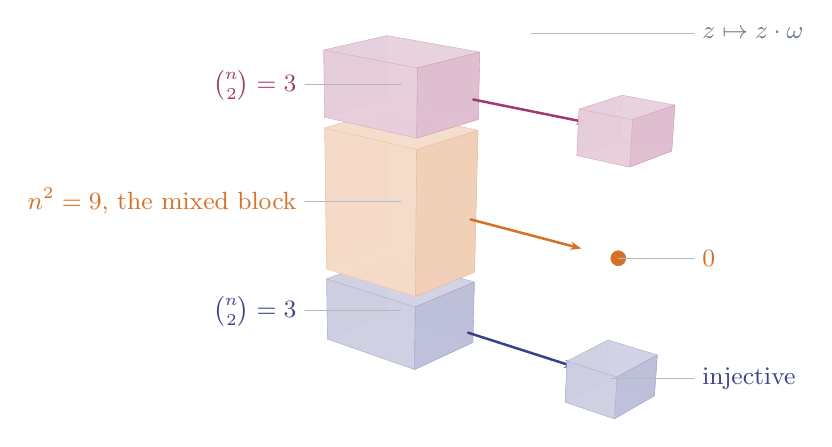
\begin{tikzpicture}[x=1cm,y=1cm,line join=round,line cap=round,
  font=\small,text=PInk]
  \path[draw=PIndigo!50!white,line width=0.12pt,fill opacity=0.88,fill=PIndigo!34!white] (-0.6495,-0.4082) -- (0.1006,-0.0954) -- (0.1020,0.6419) -- (-0.6593,0.3543) -- cycle;
  \path[draw=PIndigo!41!white,line width=0.12pt,fill opacity=0.88,fill=PIndigo!25!white] (0.1006,-0.0954) -- (1.1974,-0.4518) -- (1.2156,0.3142) -- (0.1020,0.6419) -- cycle;
  \path[draw=PIndigo!39!white,line width=0.12pt,fill opacity=0.88,fill=PIndigo!23!white] (-0.6495,-0.4082) -- (0.4577,-0.7944) -- (1.1974,-0.4518) -- (0.1006,-0.0954) -- cycle;
  \path[draw=PAmber!50!white,line width=0.12pt,fill opacity=0.88,fill=PAmber!34!white] (-0.6610,0.4824) -- (0.1023,0.7657) -- (0.1057,2.4930) -- (-0.6841,2.2726) -- cycle;
  \path[draw=PAmber!41!white,line width=0.12pt,fill opacity=0.88,fill=PAmber!25!white] (0.1023,0.7657) -- (1.2187,0.4429) -- (1.2615,2.2418) -- (0.1057,2.4930) -- cycle;
  \path[draw=PIndigo!39!white,line width=0.12pt,fill opacity=0.88,fill=PIndigo!23!white] (-0.6593,0.3543) -- (0.4649,-0.0012) -- (1.2156,0.3142) -- (0.1020,0.6419) -- cycle;
  \path[draw=PAmber!39!white,line width=0.12pt,fill opacity=0.88,fill=PAmber!23!white] (-0.6610,0.4824) -- (0.4662,0.1321) -- (1.2187,0.4429) -- (0.1023,0.7657) -- cycle;
  \path[draw=PIndigo!41!white,line width=0.12pt,fill opacity=0.88,fill=PIndigo!25!white] (-0.6495,-0.4082) -- (0.4577,-0.7944) -- (0.4649,-0.0012) -- (-0.6593,0.3543) -- cycle;
  \path[draw=PIndigo!50!white,line width=0.12pt,fill opacity=0.88,fill=PIndigo!34!white] (0.4577,-0.7944) -- (1.1974,-0.4518) -- (1.2156,0.3142) -- (0.4649,-0.0012) -- cycle;
  \path[draw=PMag!50!white,line width=0.12pt,fill opacity=0.88,fill=PMag!34!white] (-0.6858,2.4105) -- (0.1060,2.6259) -- (0.1076,3.4452) -- (-0.6968,3.2616) -- cycle;
  \path[draw=PMag!41!white,line width=0.12pt,fill opacity=0.88,fill=PMag!25!white] (0.1060,2.6259) -- (1.2648,2.3804) -- (1.2851,3.2359) -- (0.1076,3.4452) -- cycle;
  \path[draw=PAmber!39!white,line width=0.12pt,fill opacity=0.88,fill=PAmber!23!white] (-0.6841,2.2726) -- (0.4833,1.9992) -- (1.2615,2.2418) -- (0.1057,2.4930) -- cycle;
  \path[draw=PMag!39!white,line width=0.12pt,fill opacity=0.88,fill=PMag!23!white] (-0.6858,2.4105) -- (0.4846,2.1433) -- (1.2648,2.3804) -- (0.1060,2.6259) -- cycle;
  \path[draw=PAmber!41!white,line width=0.12pt,fill opacity=0.88,fill=PAmber!25!white] (-0.6610,0.4824) -- (0.4662,0.1321) -- (0.4833,1.9992) -- (-0.6841,2.2726) -- cycle;
  \path[draw=PAmber!50!white,line width=0.12pt,fill opacity=0.88,fill=PAmber!34!white] (0.4662,0.1321) -- (1.2187,0.4429) -- (1.2615,2.2418) -- (0.4833,1.9992) -- cycle;
  \draw[PIndigo,line width=0.9pt,-{Stealth[length=4pt]}] (1.1357,-0.3273) -- (2.4999,-0.7649);
  \path[draw=PMag!39!white,line width=0.12pt,fill opacity=0.88,fill=PMag!23!white] (-0.6968,3.2616) -- (0.4927,3.0334) -- (1.2851,3.2359) -- (0.1076,3.4452) -- cycle;
  \path[draw=PMag!41!white,line width=0.12pt,fill opacity=0.88,fill=PMag!25!white] (-0.6858,2.4105) -- (0.4846,2.1433) -- (0.4927,3.0334) -- (-0.6968,3.2616) -- cycle;
  \path[draw=PMag!50!white,line width=0.12pt,fill opacity=0.88,fill=PMag!34!white] (0.4846,2.1433) -- (1.2648,2.3804) -- (1.2851,3.2359) -- (0.4927,3.0334) -- cycle;
  \path[draw=PIndigo!41!white,line width=0.12pt,fill opacity=0.88,fill=PIndigo!25!white] (2.8855,-0.9288) -- (3.5029,-1.1278) -- (3.5393,-0.6113) -- (2.9148,-0.4220) -- cycle;
  \draw[PAmber,line width=0.9pt,-{Stealth[length=4pt]}] (1.1681,1.1111) -- (2.5752,0.7409);
  \path[draw=PIndigo!50!white,line width=0.12pt,fill opacity=0.88,fill=PIndigo!34!white] (2.3683,-1.2091) -- (2.8855,-0.9288) -- (2.9148,-0.4220) -- (2.3932,-0.6887) -- cycle;
  \path[draw=PIndigo!39!white,line width=0.12pt,fill opacity=0.88,fill=PIndigo!23!white] (2.3683,-1.2091) -- (2.9939,-1.4214) -- (3.5029,-1.1278) -- (2.8855,-0.9288) -- cycle;
  \path[draw=PIndigo!39!white,line width=0.12pt,fill opacity=0.88,fill=PIndigo!23!white] (2.3932,-0.6887) -- (3.0261,-0.8907) -- (3.5393,-0.6113) -- (2.9148,-0.4220) -- cycle;
  \path[draw=PIndigo!50!white,line width=0.12pt,fill opacity=0.88,fill=PIndigo!34!white] (2.9939,-1.4214) -- (3.5029,-1.1278) -- (3.5393,-0.6113) -- (3.0261,-0.8907) -- cycle;
  \draw[PMag,line width=0.9pt,-{Stealth[length=4pt]}] (1.2024,2.6340) -- (2.6552,2.3401);
  \path[draw=PIndigo!41!white,line width=0.12pt,fill opacity=0.88,fill=PIndigo!25!white] (2.3683,-1.2091) -- (2.9939,-1.4214) -- (3.0261,-0.8907) -- (2.3932,-0.6887) -- cycle;
  \node[circle,fill=PAmber,draw=white,line width=0.5pt,inner sep=2.2pt] at (3.0440,0.6175) {};
  \path[draw=PMag!41!white,line width=0.12pt,fill opacity=0.88,fill=PMag!25!white] (3.0618,2.1156) -- (3.7221,1.9785) -- (3.7633,2.5621) -- (3.0948,2.6865) -- cycle;
  \path[draw=PMag!50!white,line width=0.12pt,fill opacity=0.88,fill=PMag!34!white] (2.5180,1.9224) -- (3.0618,2.1156) -- (3.0948,2.6865) -- (2.5461,2.5111) -- cycle;
  \path[draw=PMag!39!white,line width=0.12pt,fill opacity=0.88,fill=PMag!23!white] (2.5180,1.9224) -- (3.1879,1.7756) -- (3.7221,1.9785) -- (3.0618,2.1156) -- cycle;
  \path[draw=PMag!39!white,line width=0.12pt,fill opacity=0.88,fill=PMag!23!white] (2.5461,2.5111) -- (3.2244,2.3777) -- (3.7633,2.5621) -- (3.0948,2.6865) -- cycle;
  \path[draw=PMag!50!white,line width=0.12pt,fill opacity=0.88,fill=PMag!34!white] (3.1879,1.7756) -- (3.7221,1.9785) -- (3.7633,2.5621) -- (3.2244,2.3777) -- cycle;
  \path[draw=PMag!41!white,line width=0.12pt,fill opacity=0.88,fill=PMag!25!white] (2.5180,1.9224) -- (3.1879,1.7756) -- (3.2244,2.3777) -- (2.5461,2.5111) -- cycle;
  \draw[PRule,line width=0.35pt] (-0.9368,2.8187) -- (0.2890,2.8187);
  \node[text=PMag,anchor=east,inner sep=0pt] at (-1.0368,2.8187) {$\binom{n}{2}=3$};
  \draw[PRule,line width=0.35pt] (-0.9368,1.3445) -- (0.2811,1.3445);
  \node[text=PAmber,anchor=east,inner sep=0pt] at (-1.0368,1.3445) {$n^{2}=9$, the mixed block};
  \draw[PRule,line width=0.35pt] (-0.9368,-0.0507) -- (0.2735,-0.0507);
  \node[text=PIndigo,anchor=east,inner sep=0pt] at (-1.0368,-0.0507) {$\binom{n}{2}=3$};
  \draw[PRule,line width=0.35pt] (4.0033,3.4751) -- (1.9437,3.4751);
  \node[text=PSlate,anchor=west,inner sep=0pt] at (4.1033,3.4751) {$z\mapsto z\cdot\omega$};
  \draw[PRule,line width=0.35pt] (4.0033,0.6175) -- (3.0440,0.6175);
  \node[text=PAmber,anchor=west,inner sep=0pt] at (4.1033,0.6175) {$0$};
  \draw[PRule,line width=0.35pt] (4.0033,-0.9104) -- (2.9535,-0.9104);
  \node[text=PIndigo,anchor=west,inner sep=0pt] at (4.1033,-0.9104) {injective};
\end{tikzpicture}
\end{document}
